\iffalse
\documentclass[journal,10pt]{article}
\usepackage{graphicx}
\usepackage[margin=0.5in]{geometry}
\usepackage[cmex10]{amsmath}
\usepackage{array}
\usepackage{booktabs}
\usepackage{listings}
\title{\textbf{Optimization Assignment - Linear}}
\author{Bhavani Kanike}
\date{October 2022}

\providecommand{\norm}[1]{\left\lVert#1\right\rVert}
\providecommand{\abs}[1]{\left\vert#1\right\vert}
\let\vec\mathbf
\newcommand{\myvec}[1]{\ensuremath{\begin{pmatrix}#1\end{pmatrix}}}
\newcommand{\mydet}[1]{\ensuremath{\begin{vmatrix}#1\end{vmatrix}}}
\providecommand{\brak}[1]{\ensuremath{\left(#1\right)}}

\begin{document}


\maketitle


\section*{Problem}
\fi
A factory manufactures two types of screws , A and B. Each type screw requires the use of two machines , an automatic and a hand operated. It takes 4 minutes on the automatic and 6 minutes on hand operated machines to manufacture a package of screws A,while it takes 6 minutes on automatic and 3 minutes on the hand operated machines to manufacture a package of screws B. Each machine is available for at the most 4hrs on any day. The manufacturer can sell a package of screws A at a profit of Rs. 7 and screws B at a profit of Rs. 10. Assuming that he can sell all the screws he manufactures, how many packages of each type should the factory owner produce in a day in order to maximise his profit? Determine the maximum profit.
\\
\solution
\iffalse

\section*{Solution}
Let's assume that
\begin{center}
Number of Screws A be x\\
Number of Screws B be y\\
\end{center}
\fi
The given information is summarized in Table 
		\ref{table:12/12/2/5}
\begin{table}[!ht]
	\centering
\begin{tabular}{|c|c|c|c|c|}
	\hline
	\textbf{Item}&\textbf{Number}&\textbf{Machine A}&\textbf{Machine B}&\textbf{Profit}\\
	\hline
	Screw A&x&4(min)&6(min)&7\\
	\hline
	SCREW B&y&6(min)&3(min)&10\\
	\hline
	Max.Time available& &4 hrs&4 hrs&\\
	\hline
\end{tabular}
	\caption{}
		\label{table:12/12/2/5}
\end{table}
resulting in the following optimization problem.
\iffalse
According to Question : \\\\
Automated machine works on Screw A - 4 min\\
Automated machine works on Screw B - 6 min\\\\
Miximum time - 4hrs = 4 x 60 = 240 min\\\\
Therefore,
\begin{align}
	\myvec{4 &6}\myvec{x\\y} \leq 240
\end{align}
\begin{align}
	\myvec{2&3} \myvec{x\\y} \leq 120	
\end{align}
\begin{align}
	x \geq 0 , y \geq 0
\end{align}

Hand Operated machine works on Screw A - 6 min\\
Hand Operated machine works on Screw B - 3 min\\\\
Maximum time - 4 hrs = 4 x 60 = 240 min

\begin{align}
	\myvec{6 &3}\myvec{x\\y} \leq 240
\end{align}
\begin{align}
	\myvec{2&1}\myvec{x\\y} \leq 80
\end{align}
\begin{align}
	x\geq 0 , y\geq 0
\end{align}
\\
As we need to maximize the profit ,\\
the function used here is z \\
Profit on Screw A - Rs.7\\
Profit on Screw B - Rs.10\\
Therefore,
\fi
\begin{align}
	z = \max_{\vec{x}}\myvec{7&10}\myvec{x}
	\\
	s.t. \quad
	\myvec{2&3 \\ 2 & 1} \preceq \myvec{120 \\ 80}
	\\
	\vec{x} \succeq  \vec{0}
\end{align}
%
The maximum profit is obtained as
\begin{align}
	\myvec{2&3&120\\2&1&80} \longrightarrow {R_2 - R_1} \myvec{2&3&120\\0&-2&-40} \longrightarrow{R_2*\frac{-1}{2}} \\ 
	\myvec{2&3&120\\0&1&20} \longrightarrow{R_1-3R_2} \myvec{2&0&60\\0&1&20} \longrightarrow{\frac{R_1}{2}} \myvec{1&0&30\\0&1&20}
\end{align}
yielding the maximum profit 
\begin{align}
	z = 410
\end{align}
at
\begin{align}
	\vec{x} = \myvec{30 \\ 20}.  
\end{align}
This is verified by Table 
		\ref{table:12/12/2/5/1}, where the corner points are obtained from Fig. 
		\ref{fig:12/12/2/5}.

	\begin{figure}[!ht]
		\centering
		\includegraphics[width=\columnwidth]{12/12/2/5/figs/op1.pdf}
		\caption{}
		\label{fig:12/12/2/5}
  	\end{figure}
	\iffalse
	From Fig.
		\ref{fig:12/12/2/5},
		the corner points are obtained in Table 
		\ref{table:12/12/2/5/1}.
		\fi
\begin{table}[!ht]
\begin{tabular}{|c|c|}
	\hline
	\textbf{Corner points}&\textbf{Value of Z}\\
	\hline
	(0,40)&400\\
    \hline
	(30,20)&410\\
	\hline
	(40,0)&280\\
	\hline
\end{tabular}
	\caption{}
		\label{table:12/12/2/5/1}
\end{table}
\iffalse
Hence ,Profit will be maximum if the company produces\\
30 Packages of Screw A\\
20 Packages of Screw B\\\\
Maximum Profit = Rs.410
\section*{Construction}
\begin{figure}[h]
\includegraphics[scale=0.5]{op1.pdf} 
\end{figure}
\section*{Execution}
Verify the above proofs in the following code.\\
\begin{lstlisting}
https://github.com/bhavani360/FWC_assignments
\end{lstlisting}
 \bibliographystyle{ieeetr}
\end{document}
\fi
